\chapter{Implementation}

\section{How to Apply an Aspect}

Since an aspect is a .NET attribute, it can be used just like any other attribute. But code annotated with an aspect is special in that it can be understood only by Buffalo.

An aspect can be applied in three level:

1. Method level - an individual method.
2. Class level - if applied to a class, all public methods including the public properties automatically get applied.
3. Assembly level - if applied to an assembly, \#2 will apply but for all the public classes within the assembly.

An aspect can also be excluded on any given level. If excluded the target and any nested children will be skipped over. 

No matter how the aspect is applied, ultimately it will result in a list of the methods that will be annotated. This simply mean if the aspect is applied to a single method, that method is the only one that will get MSIL modified. If the aspect is applied on the whole assembly, then all public methods will be MSIL modified.

To get the list of the eligible methods for MSIL modification, Buffalo attempts various checking according to figure~\ref{logical_inclusion} to see if it should include a given method.

\begin{figure}[H]
  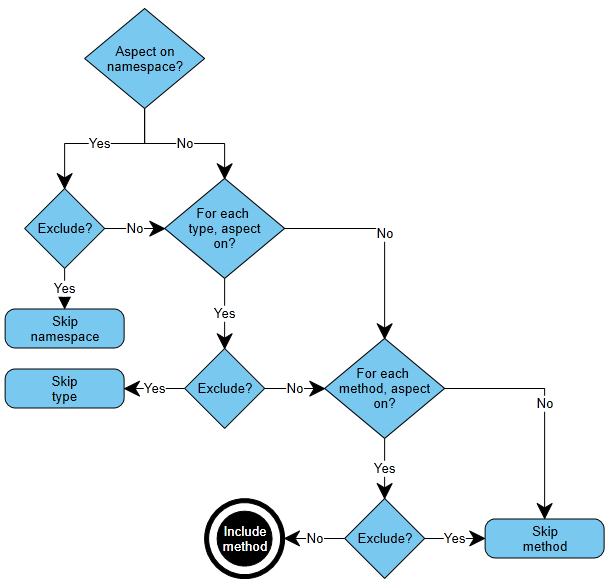
\includegraphics[scale=1.0]{AspectLogicalInclusion.PNG}
  \centering
  \caption{Logical Inclusion\label{logical_inclusion}}
\end{figure}

If no aspect is applied on the assembly, that does not necessarily mean no aspect is applied anywhere, the aspect might still be applied on any given class or method.

The take away from the above diagram, is that Buffalo first checks if an aspect is applied to the target, then check if it is set to be excluded. At the end it will end up with a list of methods that should be MSIL modified.

\section{Aspect Interface}

Figure~\ref{uml01} depicts part of the system, where it shows how we can use it to find aspects during reflection.

\begin{figure}[H]
  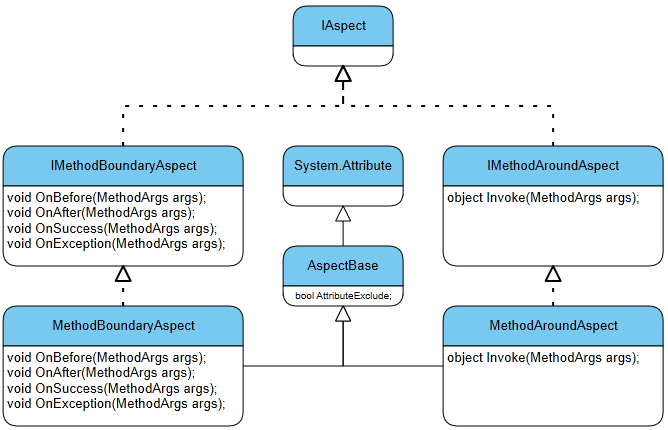
\includegraphics[scale=1.0]{Uml01.PNG}
  \centering
  \caption{Aspect Inheritance\label{uml01}}
\end{figure}

All aspects ultimately implements the IAspect interface, therefore we can conclude that for all the types in an assembly, if it implements IAspect, then it must be an aspect itself.

All aspects have a property named AttributeExclude, if set to true then the annotated target will not be included in the weaving.

Buffalo also support more than one aspect applied at any given level. This will allow developers more flexibility while developing multiple aspects and applying them as needed.

Furthermore, by default, an aspect will be automatically excluded from applying to itself. This is implemented to prevent stack overflow in some cases. Although we can argue that an aspect should be able to be applied to a different aspect, however that is not currently implemented in Buffalo.

\section{MethodArgs}

As mentioned above, when its all said and done, an aspect ultimately gets injected into an individual method. When developing an aspect, a developer can access various information about the target method, via the MethodArgs object passed in as parameter to the aspect. Currently the full method signature, the method name, return type and parameter list including parameter name, type and value are captured for each target method.

The parameter list capturing is especially interesting, it enables developer to peek inside of the method that is executing at various point and inspect its parameter values. This will be useful in case of exception handling, where it will be useful to actually see what the values were at the time of the exception.

\section{Visual Studio Solution Structure}

Originally Buffalo was in one executable, that includes the various aspects and the program that initiate the weaving. It was later on separated into two assembly. One is the actual implementation as a DLL, another is just a command line executable that calls into the DLL to perform the weaving, as shown in figure~\ref{solutionexplorer}. This separation is necessary so developer can perform weaving from the command line or hook into MS-Build if necessary. To actually write the aspect, developer only need to reference the DLL which is much cleaner than referencing an executable.

\begin{figure}[H]
  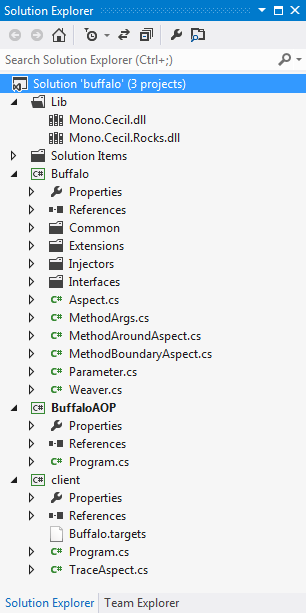
\includegraphics[scale=1.0]{SolutionExplorer.PNG}
  \centering
  \caption{Solution Structure\label{solutionexplorer}}
\end{figure}

The client project is just a test client included in the solution for testing. The full source code is included in Appendix B.

\section{Implementation Overview}

The overall implementation process can be illustrated as figure~\ref{implementation_overview}, where the first step of finding all eligible methods using the logical diagram mentioned in figure~\ref{logical_inclusion}.

\begin{figure}[H]
  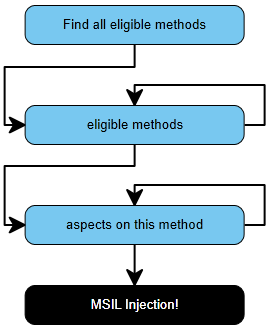
\includegraphics[scale=1.0]{ImplementationOverview3.PNG}
  \centering
  \caption{Implementation Overview\label{implementation_overview}}
\end{figure}

The actual injection phrase will be depending on the type of aspect, as we mentioned above currently Buffalo supports the MethodBoundaryAspect where various point of execution can be intercepted, and the MethodAroundAspect where a method can be completely replaced.

\section{MethodBoundaryAspect Implementation Detail}

Each type of aspect has its own injector that implements the IInjectable interface. This interface contains only one method contract - Inject(..). It takes the list of eligible methods and inject the appropriate aspect to them.

The Boundary aspect is pretty straightforward to implement, take the following hello world example, wrapped in a try..catch..finally block as we mentioned above:

\begin{lstlisting}[caption={SayHello function}, label=sayhello]
public void SayHello()
{
   try{
       Console.WriteLine(“Hello World!”);
   }catch(Exception ex){
   }finally{
   }
}
\end{lstlisting}

If we look at the generated MSIL shown in figure~\ref{methodboundaryB4}. For ease of display I have cleaned up the MSIL a bit:

\begin{lstlisting}[caption={MSIL generated for sample C\# function}, label=methodboundaryB4]
.try
{
   .try
   {
      IL_0002: Ldstr "Hello World!"
      IL_0007: call void [mscorlib]System.Console::WriteLine(string)
      IL_000e: leave.s IL0015
   }
   catch [mscorlib]System.Exception
   {
      IL_0010: stloc.0
      IL_0013: leave.s IL_0015
   }
   IL_0015: leave.s IL_001c
}
finally
{
   IL_001a: endfinally
}
IL_001c: ret
\end{lstlisting}

This is the standard emission of the CLR when it encounters the try-catch-finally statement. In CLR there is a concept of the protected region, where each region is associated with a handler. A try-catch-finally is actually encapsulated in two such regions: a catch and a finally. From here we can easily figure out where to inject our various boundary aspects, as shown in the following figure~\ref{methodboundary02}

\begin{figure}[H]
  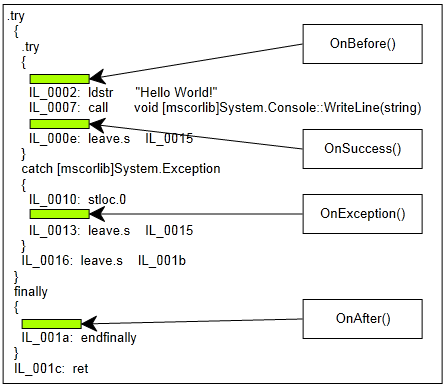
\includegraphics[scale=1.0]{MethodBoundaryOverview.PNG}
  \centering
  \caption{MSIL Interception Points\label{methodboundary02}}
\end{figure}

\section{MethodAroundAspect Implementation Detail}

The Around aspect on the other hand is a much more complicated compared to the Boundary aspect.

MethodAroundAspect implements IMethodAroundAspect that has the following contract:

void Invoke(MethodArgs arg)

From a developer’s perspective, when writing an aspect, he can issue a Proceed() to signal a call back into the original method. The steps taken to implement Around in MSIL is roughly as follow:

1. Create a replacement for the annotated function.
2. Create and store a variable pointing to the aspect.
3. Copy all parameters from original method to the newly created replacement function.
4. Create a variable to hold MethodArgs.
5. Issue a call to Invoke() from the replacement function, passing in the MethodArgs variable.
6. Handle the return value appropriately.
   6a. If original method returns non void type, store the return value appropriately.
   6b. If original method returns void, we need to discard the return value from Invoke()
7. Handle Proceed() that might be issued from inside the Invoke()
   7a. Load all the parameters onto the stack.
   7b. Call back into the original method.
   7c. Handle the return value appropriately.
8. Modify all calls from original method to the replacement method.

As figure~\ref{around_overview} shown, the actual calling of either the original or replacement method is abstracted away. This is also a testament of the saying in Software Engineering that “Anything can be resolved by another layer of abstraction”.

\section{MethodArgs}

Another early decision was that from a given aspect, developer must be able to access information about the annotated method. Details such as the name of the method; its signature and return type. Also the list of parameters that are being passed into the method including type, name and value.

Being able to capture some information about the annotated methods will be useful. For example, if we create a trace aspect to perform profiling, we can output all those information about the method at the time it was access. Being able to look at the parameter values in case of error will also be extremely useful in case of debugging.

To achieve the above MethodArgs is used. This is the object passed into each aspect. During the weaving, an instance of MethodArgs is injected into each method, with all properties assembled dynamically to capture the information of the current method.

At first each OnBefore, OnSuccess, OnException and OnAfter has its own distinct MethodArgs object passed into them. Later on as an optimization only one instance is instantiated at the beginning of the method body and that instance is used in all the MethodBoundaryAspect.

An example of how to use MethodArgs is presented in Appendix B.
%
%\begin{itemize}
%\item{} Software details (use as many section as needed for class design, 
%database tables, middleware, etc.)

%\item{} Make sure you present and comment on any interesting issues about
%your implementation that you are proud of or unhappy with

%\item{} Skip code listing and specific UML diagrams, etc. to an appendix

%\end{itemize}
%
